\documentclass[11pt]{article}
\pdfoutput=1
\usepackage{simplemargins}
\usepackage{url}
\usepackage[pdftex]{graphicx}
\usepackage{setspace}
\graphicspath{{figures/}}
\usepackage{siunitx}
\setlength{\parindent}{0pt} 
\setlength{\parskip}{1.6ex} 
\setallmargins{1in} 
\linespread{1.6}
\usepackage[round]{natbib}
\listfiles

\begin{document}

% Title must be 150 characters or less
\begin{flushleft} 
\singlespacing
{\Large \textbf{The genetic architecture of local adaptation I: The genomic landscape of 
foxtail pine (\textit{Pinus balfouriana} Grev. \& Balf.)}}
% Insert Author names, affiliations and corresponding author email.
\null

Christopher J.\ Friedline$^{1}$, 
Brandon M. Lind$^{1}$,
Erin M. Hobson,$^{1}$,
Douglas E. Harwood$^{1}$, 
Annette Delfino Mix$^{2}$,
Patricia E. Maloney$^{3}$, and
Andrew J. Eckert$^{1,4}$
\null

\bf{1} Department of Biology, Virginia Commonwealth University, Richmond, VA 23225
\\
\bf{2} Institute of Forest Genetics, USDA Pacific Southwest Research Station, Placerville, 
CA 95667
\\
\bf{3} Department of Plant Pathology, University of California, Davis, CA 95616
\\
\bf{4} Author for Correspondence
\null

$\ast$ E-mail: aeckert2@vcu.edu
\end{flushleft}

\section*{Abstract}

\section*{Introduction}
The genetic architecture of fitness-related traits has been a major focus of geneticists for 
over a century \citep[reviewed by][]{Ellegren:2008}. Genetic architecture refers to the number, type, effect size, genomic organization, 
interactions, and environmental dependency of the loci contributing to phenotypic variation 
which in turn creates variation in fitness among individuals within populations \citep[cf.][]{Eckert:2012a}. 
Interest in this architecture stems from the want to explain the nature of genetic variation which 
contributes to evolution via the accumulation of adaptations within lineages (i.e. adaptive evolution).
Early efforts to understand the genetic architecture of fitness-related traits
focused primarily on the number and effect size of the loci underlying heritable, phenotypic variation \citep{Fisher:1930}. Recent work has extended this line of research, with myriad studies linking phenotypic with genetic variation 
through linkage mapping, both within pedigrees \citep{Mauricio:2001, Neale:2011, Ritland:2011} and within 
natural populations \citep{Ingvarsson:2011, Eckert:2013a}, 
and through quantitative genetic experimentation \citep{Anderson:2013a, Anderson:2013b, Fournier-Level:2013}. Relatively 
little empirical work, however, has focused on the genomic organization of loci contributing to fitness differences 
among individuals \citep[but see][]{Stevison:2011}. This is despite clear theoretical predictions relating the evolution of the genetic architecture to the 
genomic organization of the loci comprising that architecture \citep{Kirkpatrick:2006, Yeaman:2011, Yeaman:2013}.

Evidence for adaptive evolution among populations of plants is commonly documented at both the phenotypic 
and molecular levels \citep{Kawecki:2004, Pannell:2013}, so that some of the best
examples of adaptive evolution within lineages comes from the field of plant genetics.
Adaptive evolution has been extensively documented for forest trees, especially conifers, with many instances of local adaptation clearly
being documented over the past century \citep{White:2007, Neale:2011}. Despite great advances in experimental technology, empirical 
focus has remained almost fully on the number, effect size, type, and interactions among loci contributing 
to adaptive evolution \citep{Neale:2011, Alberto:2013}.  A thorough examination of the 
genetic architecture of fitness-related traits, however, should also include 
an examination of the genomic organization of the loci contributing to trait variation. Here, we leverage 
this idea in the first of a series of papers dissecting the genetic architecture of fitness-related 
traits in a non-model conifer species, foxtail pine (\textit{Pinus balfouriana} Grev. \& Balf.), with the 
ultimate goal of testing explicit evolutionary hypotheses about the genomic organization of loci 
contributing to variation in fitness-related traits.

Ideally, the genomic organization of loci contributing to variation in fitness-related traits would follow 
naturally from the production of a genome sequence (i.e., a physical map). For many taxa, especially those with 
small to modest genome sizes, this is monetarily and computationally feasible using next-generation DNA sequencing 
technologies \citep{Koboldt:2013}. For taxa with large or complex genomes, however, even the advent of next generation DNA 
sequencing does not solve the complexity and cost hurdles associated with the production of a finished genome sequence. Conifers have large and 
complex genomes \citep{Murray:1998, Ahuja:2005}, with estimated average genome sizes in \textit{Pinus} in the 
range of \SIrange{20}{30}{Gbp}. Several genome projects, each involving many laboratories, are underway or have been 
completed \citep{Mackay:2012}. Even these efforts often initially result in limited information, 
as current assemblies of the Norway spruce (\textit{Picea abies} L.) and loblolly pine (\textit{Pinus taeda} L.) genomes 
contain millions of unordered contigs with average sizes in the thousands of base pairs \citep{Nystedt:2013}. An alternative, but not mutually exclusive, approach to describing the genome of an organism 
is that of linkage mapping. In this approach, genetic markers are ordered through observations of recombination events 
within pedigrees. This approach dates to the beginning of genetics and the logic has remained relatively unchanged 
since the first linkage maps were created in \textit{Drosophila} \citep{Sturtevant:1913}.

Renewed interest in linkage maps has occurred for two reasons. First, linkage maps can be used to order contigs 
created during genome sequencing projects \citep{Mackay:2012, Martinez-Garcia:2013}. In this fashion, linkage 
maps are used to help create larger contigs from those generated during the assembly. It is these larger contigs that 
create the utility that most practicing scientists attribute to genome sequences. Second, linkage maps are relatively 
easy to produce and provide a rich context with which to interpret population and quantitative genetic patterns of variation 
\citep[e.g.][]{Eckert:2010a, Eckert:2010b, Eckert:2013a, Yeaman:2013}. They can also be used to test explicit hypotheses about 
the organization of loci contributing to adaptive evolution. For example, \citet{Yeaman:2011} developed theoretical 
predictions about the genomic organization of loci underlying patterns of local adaptation as a function of gene flow, 
so that loci contributing to local adaptation have differing spatial structure within genomes as a result of differing 
regimes of gene flow. The relevant scale \citep[\textit{sensu}][]{Houle:2011} in these mathematical formulations is that 
of recombinational distance among loci, so that when matched with an appropriate study system, 
linkage maps provide the impetus to test basic evolutionary hypotheses. In this context, future additions of finished 
genome sequences would add only to the interpretation of results.

Construction of linkage maps have a long history within forest genetics, mostly through their use in quantitative trait locus mapping \citep{Ritland:2011}. 
Conifers in particular are highly amenable to linkage mapping, with approximately 25 different species currently having some 
form of linkage map completed \citep[see Table 5-1 in][]{Ritland:2011}. Much of the amenability of conifers to linkage mapping stems from 
the early establishment of breeding populations in economically important species and from the presence of a multicellular 
female gametophyte (i.e., the megagametophyte) from which the haploid product of maternal meiosis can be observed \citep{Cairney:2007}. Indeed, many of the first linkage maps in conifers were generated from collections of 
megagametophytes made from single trees \citep{Tulsieram:1992, Nelson:1993, Kubisiak:1996}. Continued development 
of genetic marker technologies has facilitated rapid development of linkage maps across a diversity of species, with the largest maps 
generated for economically important species \citep[e.g.][] {Achere:2004, Kang:2010, Martinez-Garcia:2013}. 
The development of biologically informative markers in non-economically important conifers, however, is hampered by production costs associated
with the development of characterized  genetic markers (i.e., those with a known DNA sequence and/or function). 
The majority of this cost is in the two-step approach needed to generate biologically 
meaningful markers: polymorphism discovery via DNA sequencing of genic regions followed by genotyping of those polymorphisms \citep[cf.][]{Eckert:2013a}. As a result, the vast majority of linkage maps outside of economically important 
species are created with uncharacterized genetic markers \citep[e.g.,][]{Travis:1998}. Much of the knowledge about the genetic 
architecture of fitness-related traits outside of a handful of economically important conifer species, therefore, is about the 
number and effect size of uncharacterized genetic markers \citep{Ritland:2011}. Cost restrictions, however, have largely disappeared. 
It is now feasible to jointly discover polymorphisms and genotype samples using high-throughput DNA sequencing 
approaches, such as restriction-associated DNA sequencing \citep [RADseq; e.g.,][] {Peterson:2012}. 

The generation of dense linkage maps from RADseq data is a complex endeavor due to the inherent stochasticity
and error prone nature of these data. Recent examples in several crop species highlight the
difficulties that must be overcome with respect to missing data and errors in calling polymorphic sites 
and the resulting genotypes \citep{Pfender:2011, Ward:2013}. Despite these difficulties, RADseq has been 
successively applied to samples taken from natural populations of non-model conifer species \citep{Parchman:2012}, but has not yet 
been applied to linkage mapping in these species, so that an exploration of these methods to linkage mapping in the large and complex 
genomes of conifers is warranted. Here, we take this approach using megagametophyte arrays from four maternal trees of foxtail pine
to generate maternal linkage maps comprised of tens of thousands of markers. There are currently no published linkage 
maps for this species nor any within the subsection \textit{Balfourianae}. By doing so, we examine the inherent biases
to the generation of RADseq data in conifer genomes and how these biases affect downstream inferences of linkage maps. We subsequently discuss
the utility of our inferred linkage maps to comparative genomics within the conifers and to tests of how patterns of gene flow 
affect the genomic organization of loci underlying fitness-related traits.


\section*{Materials and Methods}

\subsection*{Focal species}
Foxtail pine is a five needle species of \textit{Pinus} classified into 
subsection \textit{Balfourianae}, section \textit{Parrya}, and subgenus \textit{Strobus} 
\citep{Gernandt:2005}. It is one of three species within subsection \textit{Balfourianae} 
\citep{Bailey:1970} and generally is regarded as the sister species to Great Basin bristlecone pine \citep[\textit{P. longaeva} D. K. Bailey; see][] 
{Eckert:2006a}. The natural range of foxtail pine encompasses two 
regional populations located within California that are separated by approximately 500 km - 
the Klamath Mountains of northern California and the Sierra Nevada of southern California 
(Figure \ref{f:Figure01_TGG}). These regional populations diverged approximately one million years ago (mya), 
with current levels of gene flow between regional populations being approximately zero 
\citep{Eckert:2008}. Within each regional population, levels of genetic diversity and the 
degree of differentiation among local stands differ, with genetic diversity being highest in 
the southern Sierra Nevada stands and genetic differentiation being the highest among the 
Klamath stands \citep{Oline:2000, Eckert:2008}. These two regional populations
have also been recognized as distinct subspecies based on numerous quantitative traits, with \textit{P. balfouriana}
subsp. \textit{balfouriana} located in the Klamath region and \textit{P. balfouriana} subsp. \textit{austrina} located in the southern
Sierra Nevada mountains \citep{Mastrogiuseppe:1980}. The two regional populations of foxtail pine 
thus represent a powerful natural experiment within which to examine the genomic organization of loci contributing to local adaptation. The first step
in using this system to test evolutionary hypotheses is the production of a
dense linkage map.

\subsection*{Sampling}
Seed collections from 141 maternal trees distributed throughout the natural range 
of foxtail pine were obtained during 2011 and 2012. Of these 141 maternal trees, 72 were sampled from the 
Klamath region, while 69 were sampled from the southern Sierra Nevada region. These 141 families were
divided among 15 local stands ($n = 4$ to $17$ trees/stand), with eight stands in the Klamath region and seven stands in the southern Sierra Nevada.
Approximately 50 seeds were germinated from each seed collection and 35 of those 50 seedlings were planted in a 
common garden located at the USDA Institute of Forest Genetics, Placerville, California. The 
common garden was established using a randomized block design and involved three separate plantings of seeds spanning
approximately one year from June 6, 2012 until May 20, 2013. Four of the 141 maternal trees were selected 
at random ($n = 2$ from the Klamath region and $n = 2$ from the southern Sierra Nevada) for linkage analysis. 
For each of these trees, \SIrange{75}{100}{} seeds were germinated and planted in the common garden. 
Upon germination, haploid megagametophyte tissue was rescued from each seedling, cleaned, and stored for further 
analysis in \SI{1.5}{\mL} Eppendorf tubes at \SI{-20}{\celsius}.

\subsection*{Library Preparation and Sequencing}
Total genomic DNA was isolated from each rescued megagametophyte using the DNeasy 96 Plant 
kit following the manufacturer’s protocol (Qiagen, Germantown, MD). RADseq \citep{Davey:2010, Parchman:2012, Peterson:2012} 
was used to generate a genome-wide set of 
single nucleotide polymorphism (SNP) markers for linkage mapping following the protocol 
outlined by \citet{Parchman:2012}. In brief, this protocol is a double digestion RADseq 
approach based on digestion of total genomic DNA using EcoRI and MseI followed by single-end 
sequencing on the Illumina HiSeq platform. Following digestion, adapters 
containing amplification and sequencing primers, as well as barcodes for multiplexing, 
were ligated on to digested DNA fragments. We chose to multiplex 96 samples using the 
barcodes available from \citet{Parchman:2012}. One of these samples, per set of 96, was a pseudo-diploid
constructed by pooling five megagametophytes sampled from the same maternal tree. We used the genotype of the
pseudo-diploid sample as that of the maternal genotype, although there is a probability of $0.5^{4} = 0.0625$ that 
the genotype for any given SNP will be mistakenly called homozygous due to the five megagametophytes all being of the same allele \citep[see][]{Morris:1978}.
These barcodes are a mixture of eight, nine, and  10 bp tags that differ by at least four bases, so as to accommodate
sample identification in the presence of sequencing errors. Following ligation, successfully ligated DNA fragments were 
amplified using PCR and amplified fragments were size selected using gel electrophoresis. We selected 
fragments in the size range of 400 bp (\SIrange{300}{500}{bp}) by excising and purifying pooled DNA from 2.5\% 
agarose gels using QIAquick Gel Extraction Kits (Qiagen). Further details, including relevant reagents and 
oligonucleotide sequences, can be found in File S1. All DNA sequencing was performed on the Illumina HiSeq 2000 or 2500
platform at the VCU Nucleic Acids Research Facility (\url{http://www.narf.vcu.edu/}).

\subsection*{DNA Sequence Analysis}
There are multiple steps involved with the processing of raw DNA sequence reads into a set of SNP genotypes that are useful for linkage mapping:
(1) quality control, filtering, and demultiplexing, (2) assembly to generate a reference sequence for mapping reads, (3) mapping 
of reads to call SNPs and genotypes for each sample, and (4) filtering of SNPs and the resulting genotypes for
data quality and biological meaning.

DNA sequence reads were demultiplexed into sample-level fastq files, following quality control 
and filtering.  The filtering pipeline was adapted from \citep{Friedline:2012fm}, and is briefly: reads 
containing any N beyond the first base were excluded. Reads having N as the first base were shifted 
to exclude it.  Additional quality filtering ensured that all reads in the resulting set for downstream 
processing had a minimum average quality score of 30 over 5 bp, overlapping windows 
and that not more than \SI{20}{\percent} of the bases had quality scores below 30. Reads passing the 
quality control steps were demultiplexed into sample-specific fastq files by exact pattern matching to 
known barcodes.

From each set of demultiplexed reads, the individual with the largest number of reads as assembled using 
Velvet (Zerbino, version 1.2.10), with hash length ($k$) coverage cutoff optimized using parameter sweeps of $k$ 
through the contributed VelvetOptimiser (\url{http://www.vicbioinformatics.com}, version 2.2.5) 
script (for odd $k$ on $k=[19,65]$).  Assembly robustness was evaluated in each case using the LAP likelihood 
framework \citep{Ghodsi:2013bc}, version 1.1.  Each assembly was also indexed and aligned 
(Figure \ref{f:mapping_performance}) to the original set of reads 
using Bowtie2 \citep{Langmead:2012jh} (\texttt{--local --very-sensitive}) and compared the average maximum 
likelihood estimate. In all cases, the assembly with the highest average maximum likelihood value was 
chosen as the reference for SNP calling.

SNPs were called for all individuals against their respective reference using a variety of methods.  First, 
reads were mapped to the reference with Bowtie2 (\texttt{--local --very-sensitive-local}).  These resulting 
sam files were converted their binary equivalent (e.g., bam) using \texttt{samtools} version 0.1.19 
(\texttt{view, sort, index}) \citep{Li:2009ka}.  SNPs were called using \texttt{bcftools} and filtered using 
\texttt{vcfutils} to exclude SNPs with less than 100x coverage. The resulting variant call files (vcf) 
were further processed using \texttt{vcftools} version 0.1.11 (cite) to remove indels and exclude genotype 
calls below a quality threshold of 5, and output as a matrix (\texttt{--012}) of genotypes by individuals.  

We used several thresholds to filter called SNPs for linkage mapping. First, 
we excluded SNPs using a $\chi^2$ test of homogeneity against an expectation of 1:1 segregation. This segregation pattern was expected because
the maternal tree had to be a heterozygote to detect a SNP, and Mendel's first law 
guarantees that the segregation ratio for this SNP should be 1:1. Significance of each test was 
assessed using a Bonferroni-corrected significance threshold of $\alpha = 0.05$, where $\alpha$ was corrected using the number of SNPs tested. 
Second, we filtered the resulting SNPs based on the genotype of the pseudo-diploid sample so as to keep only those SNPs
where the pseudo-diploid was called a heterozygote or had a missing genotype call.
Lastly, we filtered the resulting SNPs so as keep only those that had a minimum of $5$
genotype calls for each of the alternate alleles. The resulting subset of SNPs was then used as the input to linkage analysis. 

\subsection*{Linkage Analysis}
The production of a linkage map for a single tree requires three main steps: (1) calculation of 
pairwise distances between all pairs of loci, (2) clustering (i.e., grouping) of loci based on these pairwise distances, 
and (3) ordering of loci within each cluster.  A variety of software packages exist to carry out these steps \citep[e.g.,][]{VanOoijen:2011}.
Traditional software packages for linkage mapping, however, are not amenable to large amounts of missing data and frequent
errors in genotype calls. The former causes issues with all aspects of analysis, while the latter primarily affects the 
genetic distances between markers \citep{Cartwright:2007}. We thus followed the approach of \citet{Ward:2013}, 
which was designed specifically for RADseq data. 

In brief, this method can be described as follows. Pairwise distances were estimated and loci were clustered using a 
custom R script \citep[see File S2;][]{R:2013}. We used MSTmap \citep{Wu:2008a} 
to infer marker order and Maskov \citep{Ward:2013} to impute and correct genotypes. The algorithms available
in MSTmap can also be used to impute and correct genotype errors \citep[see][]{Wu:2008a}, but the amount of missing
data and putative genotyping errors in our RADseq data far surpassed those used to develop this software. These two programs
were used in an iterative fashion. MSTmap was used initially to order markers, which was followed by the use of Maskov
to impute and correct putative genotype errors conditional on this initial marker ordering. A last round of ordering 
was performed using MSTmap conditional on the imputed and error corrected genotype data. This general schema
was followed for each of the four maternal trees independently.

The relevant pairwise distance for linkage mapping in our haploid case is the probability of observing a recombination 
event between two haplotypes. This distance can be calculated for a set of biallelic loci using the Hamming distance ($d_{i,j}$).
The Hamming distance is the number of differences separating two binary strings \citep{Hamming:1950}. 
The binary strings are the haploid genotypes for a set of two megagametophytes. 
This distance, scaled by the number of positions (i.e., $d_{i,j}/n$), 
is the maximum likelihood estimate of the probability of a recombination event with respect to a pair of haplotypes \citep{Wu:2008a}.
It is also an estimate of the recombination fraction, so that these distances can be transformed into LOD scores \citep[see][]{Morton:1955}.
This is the estimate we used to construct a matrix of pairwise distances between all possible pairs of loci passing our quality thresholds.

The matrix of pairwise distances between all possible markers was clustered using two methods: (1) hierarchical clustering with 
either Ward's method \citep{Ward:1963} or average linkage \citep{Sokal:1958} as the linkage function and (2) \textit{K}-means clustering \citep{Hartigan:1979}. We explored groupings ($K$) based on clustering on the interval $K=[8,16]$. This interval was chosen because 
it brackets the haploid chromosome number of foxtail pine ($1N = 12$). 
For hierarchical clustering, this entailed cutting the resulting dendrogram at a specific height, so that the desired number of groups resulted. For \textit{K}-means clustering
values of \textit{K} were established \textit{a priori}. Solutions in all cases were compared using silhouette plots \citep{Rousseeuw:1987}.
The value of $K$ which maximized the number of loci correctly classified  (i.e., $s_{i} \geq 0.80$ where $s_{i}$ is the 
silhouette width of individual \textit{i}) was chosen as the optimal value of the number of clusters.

Ordering of loci within clusters was carried out using MSTmap \citep{Wu:2008a}. This method takes a full, undirected graph where nodes are loci and edges are based on the values of $d_{i,j}/n$ and finds the correct order of markers based on the minimum-weighted traveling salesman path. \citet{Wu:2008a} showed that the minimum-weighted traveling salesman path
can be found using a minimum spanning tree and that this minimum-weighted traveling
salesman path corresponds to the correct order of the loci if the minimum spanning tree on
the full, undirected graph is unique. We employed MSTmap using the maximum likelihood objective function, grouping turned off, imputation of 
missing data turned off, and the Kosambi mapping function \citep{Kosambi:1944}. The resulting ordering of loci
within each cluster, along with the distances (i.e., cM) in each cluster, were taken as the initial linkage map from which
data were error corrected and imputed.
 
Data were subsequently imputed and corrected for errors using Maskov \citep{Ward:2013}. A full account of the mechanics of the algorithm
used in Maskov can be found in Text S1 from \citet{Ward:2013}. For our purposes, the accuracy of the imputation and
error correction depends upon two choices: (1) the threshold for missing data for a given megagametophyte and (2) the number of 
contiguous loci where genotype errors can occur. We chose a value equal to the $75^{th}$ percentile for the amount of 
missing data across megagametophytes for the former and a value of 5\% of the number of loci in the initial map for each
cluster for the latter.

A final round of ordering was conducted with the imputed and error corrected data using MSTmap as described previously. Imputation 
and error correction resulted in many loci where $d_{i,j}/n = 0$. These co-segregating markers were thus mapped to the same bin
\citep[see][]{Wu:2008a}. The collection of resulting ordered clusters was taken as the final linkage map for each of the for maternal trees. 
The end result of the linkage analysis was thus four independent linkage maps, one per maternal tree.

\subsection*{Sensitivity Analysis}
The production of linkage maps for each maternal tree required many assumptions.
Given that the inferred maps will be used in downstream analyses, including acting as aids
to help impute missing data in population-level sampling, we explored the effect of these assumptions on 
the resulting linkage maps using sensitivity analysis. The effect of assumptions 
were examined by modifying threshold values defining each assumption. We selected the
data from the maternal tree with the largest number of reads as the focal linkage map with which to explore
the sensitivity of our results to our assumptions.

First, we explored the effect of assumptions made during the process of read mapping to detect SNPs and call genotypes \citep[cf.][]{Pool:2010}.
The mapping of reads requires a reference against which to match reads based on their similarity. The assembly process, however, requires optimization of the hash length (see \textbf{DNA Sequence Analysis}),
which in turn affects the quality of the contigs comprising the assembly (CITATION).  
Since it is the contigs in the assembly that directly affect the ability to map reads and hence call SNPs, we explored the effect
of assembly choice on SNP calling. We selected the next best assemblies flanking the assembly identified as optimal via maximum-likelihood
and for each performed SNP calling as described previously. When loci were shared across SNP sets (see \textbf{Consensus Map 
Construction and Biological Interpretation}), we conducted linkage mapping as
described previously (i.e., we used all of the other previous thresholds unless otherwise noted) for each
set and compared the resulting maps of the shared loci using Spearman rank correlations \citep{Spearman:1904}. 
For linkage mapping, we selected the method of clustering used that defined the best 
value of \textit{K} in the previously described linkage analyses (see \textbf{Linkage Analysis}). 
The significance of each comparison was tested via permutation 
analysis ($n = 10,000$ permutations) using a Bonferroni-corrected significance threshold of $\alpha = 0.05$. Non-significant values 
were taken as evidence of significantly different orderings.

Second, we explored the use of thresholds for segregation distortion and 
use of the pseudo-diploid sample to call the maternal genotype to filter SNPs prior to linkage mapping. 
We modified the significance threshold to Bonferroni-corrected values of $\alpha = 0.01, 0.05,$ 
and $0.10$ to study the effects of segregation distortion on the resulting map. 
Lastly, we built linkage maps with and without
use of the pseudo-diploid based filtering. Comparisons among the resulting linkage maps were made
in a fully factorial design and maps were compared using pairwise Spearman correlation coefficients 
(i.e., {$6 \choose 2$} = $15$ unique comparisons). The significance of each correlation coefficient 
was tested using permutation analysis ($n = 10,000$ permutations) and a Bonferroni-corrected significance threshold of $\alpha = 0.05$. 
Non-significant values were taken as evidence of significantly different orderings.
In all cases, linkage mapping as described previously  (i.e., we used all of the other previous thresholds unless otherwise noted) 
was carried out for each of the resulting SNP sets based on the optimal assembly, with the 
method of clustering used that defined the best value of \textit{K} in the previously 
described linkage analyses (see \textbf{Linkage Analysis}). 

Lastly, we explored the thresholds used in imputation and error correction. We varied the threshold upon which
we allowed the maximum amount of missing data, as this may affect the uniqueness 
or non-uniqueness of the minimum spanning tree used during ordering of the loci. Specifically,
we examined the effects of using as the threshold, the $10^{th}$, $25^{th}$, $50^{th}$, $75^{th}$, and $95^{th}$ percentiles of
the distribution of missing data across megagametophytes. We also varied the threshold determining 
the number of consecutive loci allowed to have incorrect genotypes. Incorrect genotypes inflate estimated
map distances due the larger number of recombination events needed to explain the data. Specifically, we
examined using as thresholds, 1\%, 5\%, and 10\% of the number of loci per cluster as being erroneous. We chose to examine the effects of these threshold values in a fully factorial design 
requiring 15 treatment comparisons. As such we restricted
analysis to the largest linkage group for the maternal tree with the largest number of reads used to construct
the assembly. For each treatment combination we produced a new linkage map, and when loci were shared, we calculated
the Spearman rank correlation of all possible pairwise combinations of the $15$ orderings (i.e., {$15 \choose 2$} = $105$ unique
comparisons). The significance of each comparison was tested via permutation analysis ($n = 10,000$ permutations)
using a Bonferroni-corrected significance threshold of $\alpha = 0.05$. Non-significant values were taken as evidence of significantly different orderings.

\subsection*{Consensus Map Construction and Biological Interpretation}
The four linkage maps, one for each maternal tree, were combined into a consensus map using MergeMap \citep{Wu:2008b}. This
method uses Directed Acylic Graphs (DAGs) to merge independent linkage maps into a consensus linkage map. Prior to building the consensus 
linkage map, contigs that were shared by each map were identified through use of XXXXX.

\section*{Results}

\subsection*{DNA Sequence Analysis}

\subsection*{Linkage Mapping}

\subsection*{Sensitivity Analysis}

\subsection*{Consensus Map Construction and Biological Interpretation}


\section*{Discussion}

\section*{Acknowledgements}

The authors would like to thank the staff at the USDA Institute of Forest Genetics, the 
VCU Nucleic Acids Research Facility, and the VCU Center for High Performance Computing. 
In addition, we would like to thank Tom Blush and Tom Burt for help in obtaining 
seeds. Funding for this project was made available to AJE via start-up funds from Virginia 
Commonwealth University. CJF was supported by the National Science Foundation (NSF) National Plant Genome 
Initiative (NPGI): Postdoctoral Research Fellowship in Biology (PRFB) FY 2013 Award \#NSF-NPGI-PRFB-1306622.

\clearpage

\singlespacing
\bibliographystyle{spbasic}
\bibliography{refs}

\clearpage

\begin{figure}[t]
\centering
\includegraphics[width=1.0\textwidth]{Figure01_TGG}
\caption{Geographical locations of foxtail pine samples used to construct a common garden located in Placerville, CA. Circles
denote the 15 unique locations from which $4$ to $17$ maternal trees were sampled. Circles enclosed in squares denote
locations from which maternal trees used in linkage mapping were sampled. Photo credits: lower: T. Burt; upper: A. Delfino Mix}
\label{f:Figure01_TGG}
\end{figure}

\begin{figure}[t]
\centering
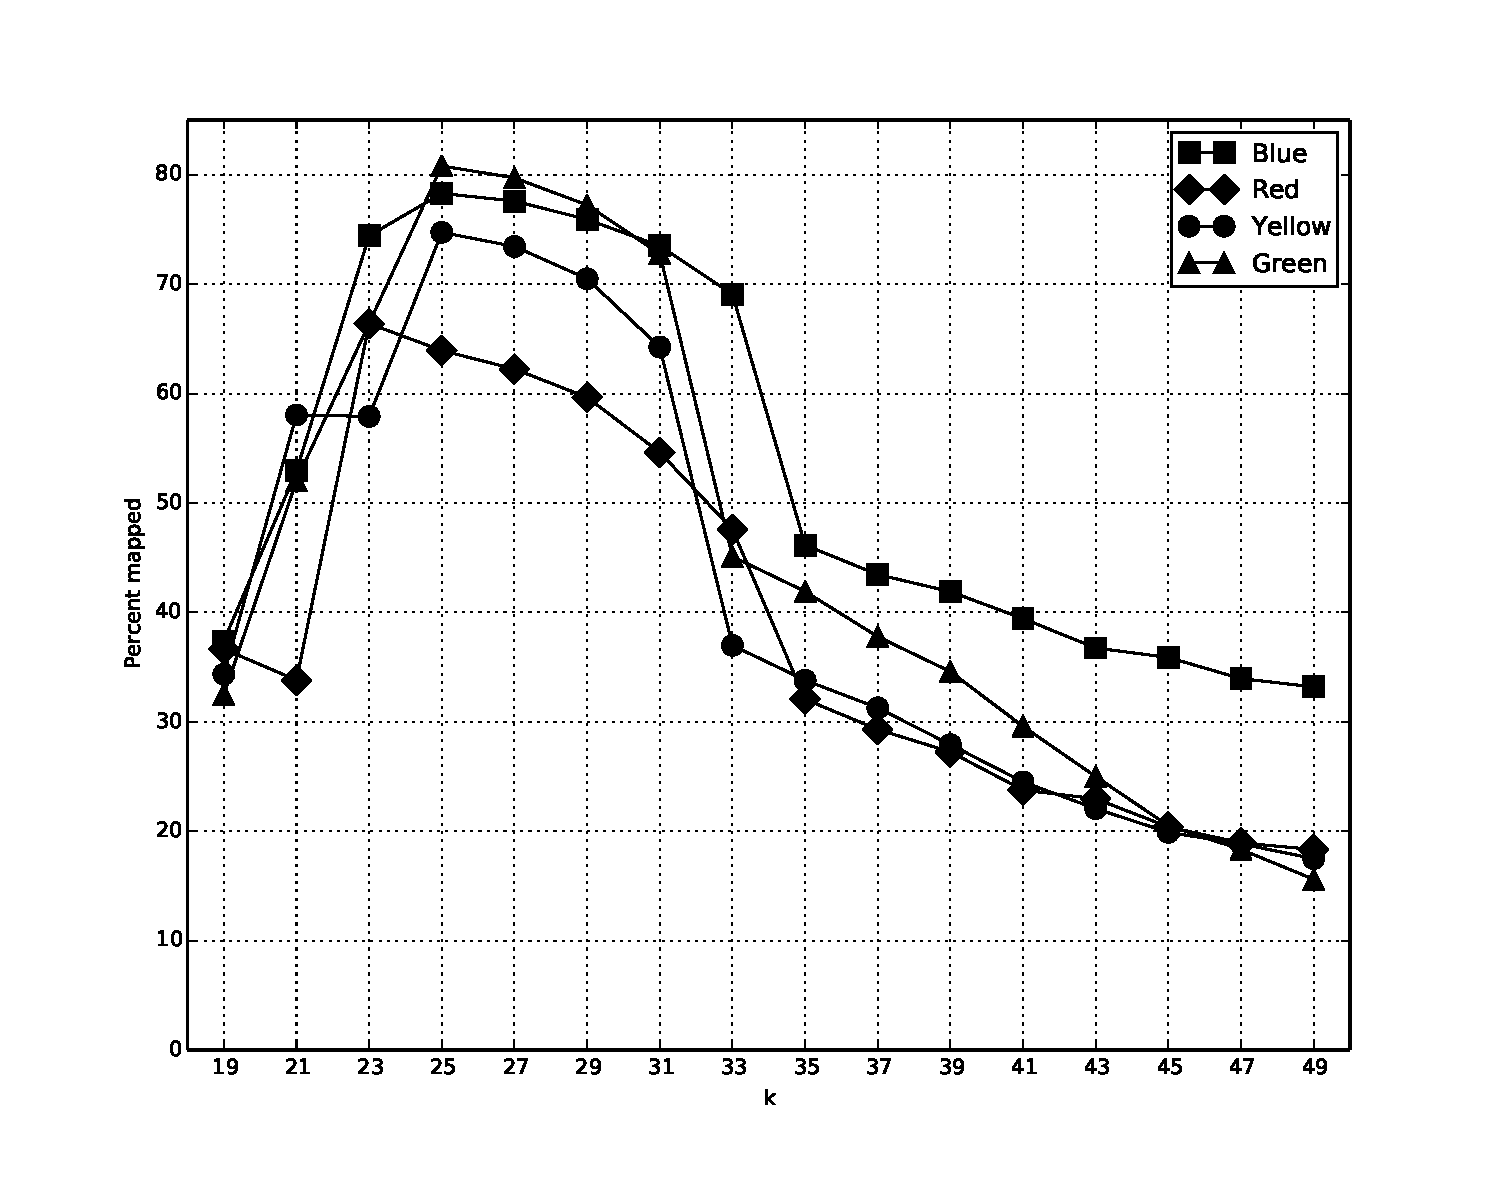
\includegraphics[width=1.0\textwidth]{mapping_performance}
\caption{Mapping performance at various sizes of $k$ for all four assemblies.  Assemblies using 
$k>53$ were excluded from the figure.}
\label{f:mapping_performance}
\end{figure}

\end{document}
